%%%%%%%%%%%%%%%%%%%%%%%%%%%%%%%%%%%%%%%%%%%%%%%%%%%%%%%%%%%%%%%%%%%%%%
% How to use writeLaTeX: 
%
% You edit the source code here on the left, and the preview on the
% right shows you the result within a few seconds.
%
% Bookmark this page and share the URL with your co-authors. They can
% edit at the same time!
%
% You can upload figures, bibliographies, custom classes and
% styles using the files menu.
%
%%%%%%%%%%%%%%%%%%%%%%%%%%%%%%%%%%%%%%%%%%%%%%%%%%%%%%%%%%%%%%%%%%%%%%

\documentclass[12pt]{article}
\usepackage{xcolor}
% Definindo novas cores
\definecolor{verde}{rgb}{0,0.5,0}
% Configurando layout para mostrar codigos C++
\usepackage{listings}
\lstset{
  language=C++,
  basicstyle=\ttfamily\small, 
  keywordstyle=\color{blue}, 
  stringstyle=\color{verde}, 
  commentstyle=\color{red}, 
  extendedchars=true, 
  showspaces=false, 
  showstringspaces=false, 
  numbers=left,
  numberstyle=\tiny,
  breaklines=true, 
  backgroundcolor=\color{green!10},
  breakautoindent=true, 
  captionpos=b,
  xleftmargin=0pt,
}
\pagestyle{empty}

\usepackage{sbc-template}

\usepackage{graphicx,url}

%\usepackage[brazil]{babel}   
\usepackage[utf8]{inputenc}  


     
\sloppy

\title{Analise de simuladores de Rede \\ }

\author{ Esdras Fragoso da Silva Neto, \\ Jessica Keyla de Sousa Silva, \\
Victor Mateus Batista de Oliveira Queiroz, \\ Antonio Ferreira de Araujo\\ 	Wellington João da Silva Sousa Júnior}


\address{Universidade Federal do Piauí - UFPI\\
 Campus Senador Helvídio Nunes de Barros \\ Bacharelado em Sistemas de Informação \\ Disciplina: Redes De Computadores II \\ Professor: Fredison Muniz De Sousa \\    
  \email{\{tonyaraujo4, victorqueirozvictoroliveira\}@outlook.com,}
  \email{\{esdrasfragoso, jessica.keylla98, wellingtonjunior199517\}@gmail.com,}
}

\begin{document} 

\maketitle


     
\begin{resumo} 
  Este trabalho descreve a utilização de dois diferentes tipos de simuladores de rede o Network Simulator – NS e o Graphical Network Simulator – GNS3. Sendo o primeiro mais voltado para pesquisa e o segundo para aplicação pratica em projetos de rede.  Utilizando o NS demostramos uma possível solução para gargalos na rede.  Já com GNS3 foi possível projetar uma estrutura de rede para uma escola, apresentando o levantamento da quantidade de equipamentos necessários, que tipo de topologia deve ser empregada, enfim ele simula uma experiência completa do desenvolvimento de uma rede física. O que se pode notar é que o NS está mais voltado pra solucionar problemas lógicos da rede, que envolva pesquisa, experimentação, calculo, ele vai trazer soluções logicas, em contrapartida o GNS3 apresenta soluções voltadas para a infraestrutura da rede, apresentando meios para testar as melhores formas de infraestrutura para determinado projeto até encontrar a melhor estrutura para implementar.    
\end{resumo}


\section{Introdução}
A utilização de simuladores em redes de computadores é um artifício engenhoso, pois, propicia a redução de riscos e custos de um projeto. Isto se deve ao fato dos simuladores conseguirem virtualizar dispositivos reais, proporcionando um estudo detalhado de  todos os periféricos da rede.

Sabendo da importância dos simuladores para área de redes, este trabalho busco apresentar dois diferentes categorias de simuladores o Network Simulator – NS e o Graphical Network Simulator – GNS3, estes dois cada um a sua maneira servem a propósitos primordiais, o primeiro atua na área de pesquisa, mas votado para sintetizar e experimentar soluções matemáticas para o aprimoramento da rede que esta sendo projetada ou estudada. Já o segundo atua auxiliando os projetistas da infraestrutura da rede, permitindo-os realizar testes de diversas estruturas e topologias de rede até encontrar a ideal para ser implementada. Desta forma é reduzido significativamente as chances de erros e desperdícios. 

O trabalho está dividido em duas partes, a primeira voltada para o NS contendo: uma descrição do NS, um tutorial de como instala-lo no sistema operacional Linux, descreveu-se um problema para ser resolvido com uso de simuladores, realização de uma simulação no NS, apresentação dos resultados obtidos com a simulação e por fim o anexo do código fonte utilizado no NS.  A segunda aborda o GNS3 onde se temos: uma descrição detalhada do GNS3, um tutorial de como instala-lo, o levantamento de uma problemática que necessita a utilização do GNS3, descrição da simulação feita no GNS3 para solucionar o problema e por fim os resultados obtidos com a simulação.   

\section{Network Simulator – NS} \label{sec:firstpage}

O NS-2 (Network Simulator versão 2) é um software gratuito e de código fonte aberto.  A topologia de simulação deve ser configurada em um script escrito em linguagem OTcl. O ns2 corresponde a segunda versão do ns, simulador de objetos discretos de uma rede, que foi concebido em 1989 a partir de uma variação do REAL Network Simulator, um projeto da Cornell University, EUA, o ns tem evoluído desde então, sempre com suporte e apoio de várias organizações.

O NS2 prevê suporte ao fluxo TCP e variantes do protocolo, multicast, roteamento, e também ao tráfego UDP. Possui um visualizador para animações de simulação (nam – network animator), e algumas ferramentas matemáticas como gerador de números aleatórios e integrais para cálculos estatísticos.

\subsection{Instalação}
A instalação do simulador ns2 foi feita no sistema operacional Linux (Ubuntu 16.04). A escolha desse sistema se deu por vários fatores, e um desses foi que o ns2 já vem pré-instalado nesse sistema.

Para a instalação, usamos um pacote fornecido pela criadora do simulador com todos os aplicativos necessários. Após baixar o arquivo, no terminal de comando foi feita a descompactação e a instalação por linha de comando.

Para confirmar a correta instalação foram feitas várias chamadas de processos relacionados com o simulador. Todos os teste foram concluídos com êxito.
\subsection{Problemática} 

Supondo que um dono de provedor de internet, se deparar com a situação de seu link não suportar a quantidade de usuários que ele esta distribuindo internet. Esta situação colocaria a credibilidade do seu negócio em risco, então imediatamente ele seria levado a tomar uma decisão para resolver o problema, mas o que ele realmente deve fazer? Aumentar o seu link? se sim para qual tamanho? instalar uma Web cache?  mas seria suficiente? Qualquer decisão que ele tomar as escuras pode ser a decisão errada e acarretar em grandes prejuízos para o seu negócio. 

Como em redes nada é uma receita de bolo pronta, cada caso tem suas peculiaridades, então precisa-se testar com bom senso todas as possibilidades até encontrar a adequada, mas o caso é que testes reais custam caro e demandam tempo. Então para solucionar tal problemática surge o simulador NS2 capaz de simular o problema e no processo apontar a solução ideal para o problema. 

\subsection{Simulação}

Para a simulação de fluxo de dados no ns2, configuramos no código OtcL as variáveis da simulação, o arquivo para coleta dos resultados, a quantidade dos nós na rede, os enlaces de cada nó, o tamanho dos pacotes, a taxa de envio e recebimento, os protocolos de transporte. O script com essas e outras configurações será compilado no nam. Esse script está anexado ao artigo.  

Como representa a figura~\ref{fig:topologia}, os links duplex entre os nós 0 e 2 e nós 1 e 2 possuem largura de banda de 5Mb por segundo (Mbps) e se propagam a uma taxa de 50 ms. No enlace entre os nós 2 e 3, nossa simulação foi configurada com a largura de banda de 1 Mbps com tempo de propagação de 100 ms. Foi criado buffers(Memória Principal) de 20 posições nos nós n2 e n3 para alocar os pacotes que não entram no enlace diretamente. Os nós n3 e n4 e n3 e n5 têm largura de 5 Mbps cada e 20 ms de tempo de propagação.  

\begin{figure}[ht]
\centering
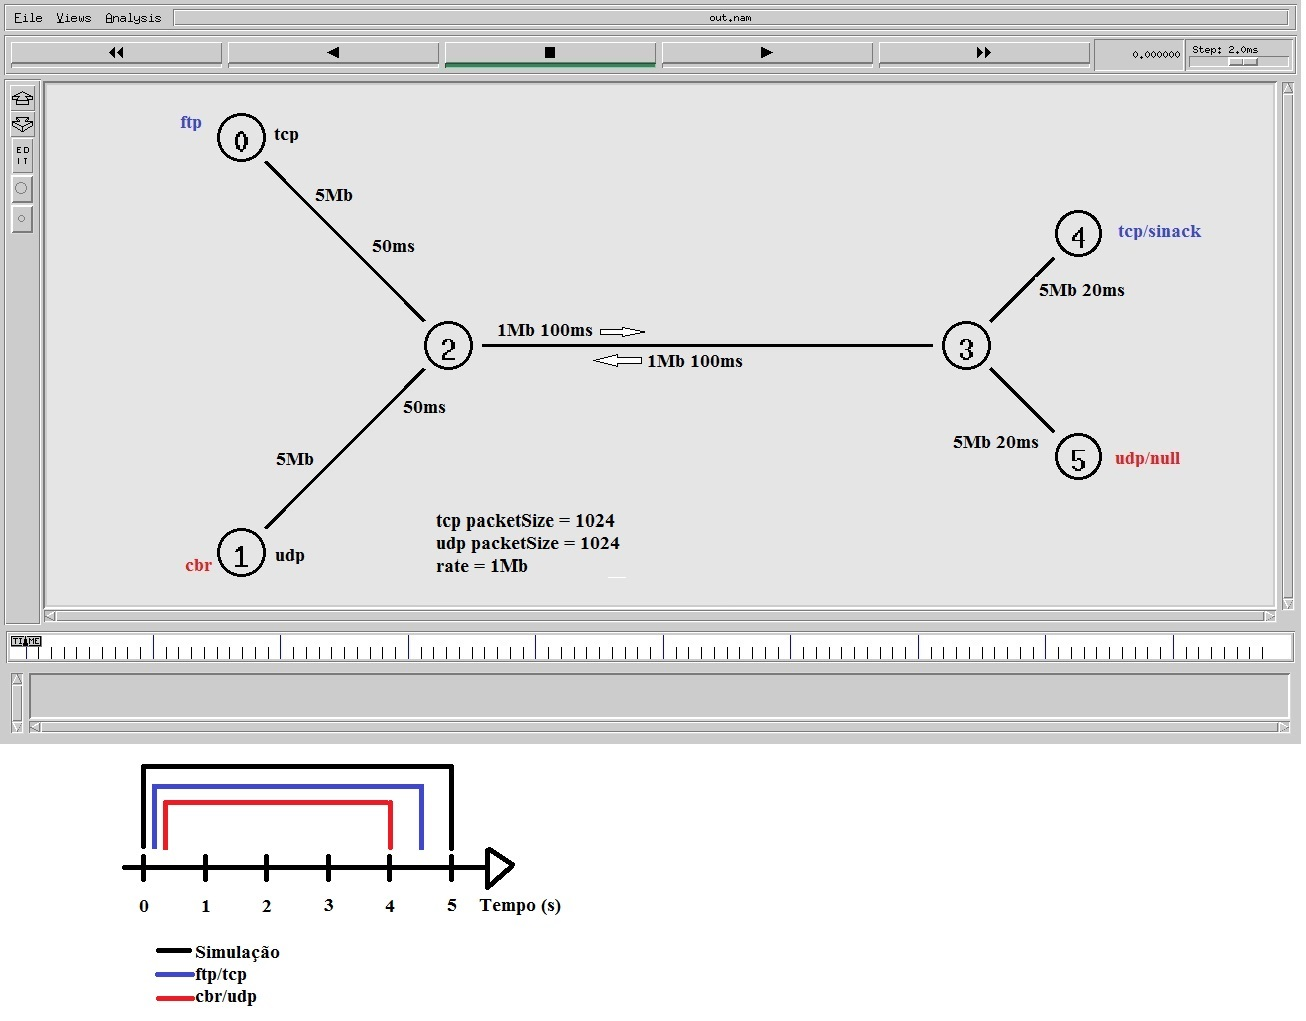
\includegraphics[width=.9\textwidth]{simulador_ns2.jpg}
\caption { Topologia da simulação}
\label{fig:topologia}
\end{figure}

O enlace n3 e n4 foi configurado para receber os pacotes FTP(File Transfer Protocol), com protocolo TCP(Transmission Control Protocol) vindos do nó n0. Também o nó n4 envia um Sinack sempre que recebe um pacote de n3.
O enlace n3 e n5 foi configurado para receber os pacotes cbr, com protocolo UDP(User Datagram Protocol) vindos do nó n1.
Então com o terminal aberto, damos o comando para iniciar a simulação. Na figura~\ref{fig:tcl} vemos a demostração do código tcl(Tool Command Language) para esta configuração.

\begin{figure}[ht]
\centering
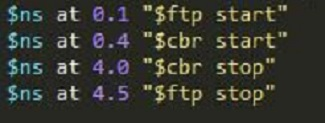
\includegraphics[width=.9\textwidth]{tcl.jpg}
\caption { tempo para start e stop dos protocolos}
\label{fig:tcl}
\end{figure}

Configuramos a simulação para o protocolo FDP começar o envio de pacotes no tempo de 0.1 s. no tempo de 0.4 o UDP com cbr começa o envio dos pacotes.

\subsection{Resultados}
Com os enlaces n0 e n2, n1 e n2  configurados com largura de 5 Mb e o enlace entre os nós n2 e n3 configurado com a banda de 1Mb, rapidamente este enlace consome toda a banda disponível, fazendo o buffer do nó n2 comecar a ser usado. Tal caso é desmostrado pela figura~\ref{fig:buffer}. 

\begin{figure}[ht]
\centering
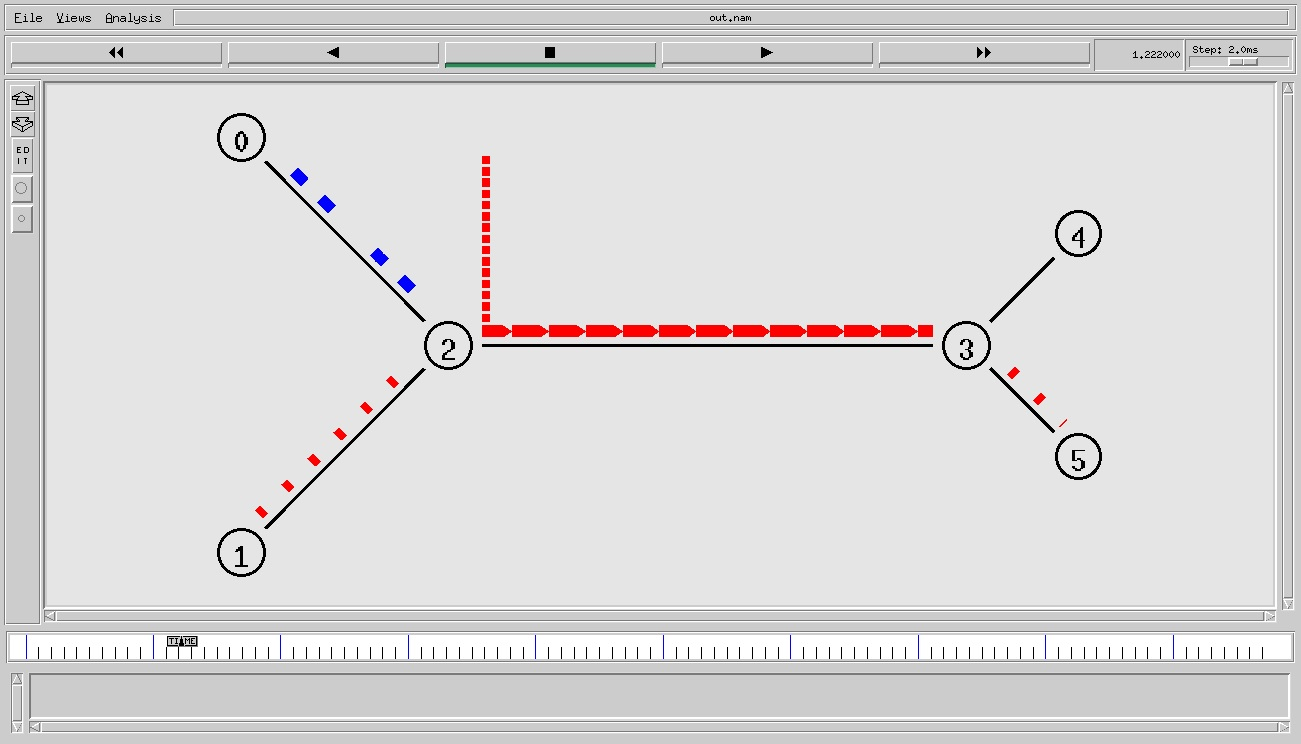
\includegraphics[width=.9\textwidth]{buffer.jpg}
\caption { Buffer de n2 em uso}
\label{fig:buffer}
\end{figure}

A banda do enlace n2 a n3 está totalmente sendo usado por pacotes vindo do udp. Como este enlace tem largura menor do que os enlaces n0 e n1, o gargalo se forma decorridos 1.2s de simulação. Este exemplo ilustrado pela figura~\ref{fig:gargalo}. Nela se apresenta a perda de pacotes que ocorre porque a largura de banda é insuficiente para fazer a distribuição dos pacotes nos nós n4 e n5.

\begin{figure}[ht]
\centering
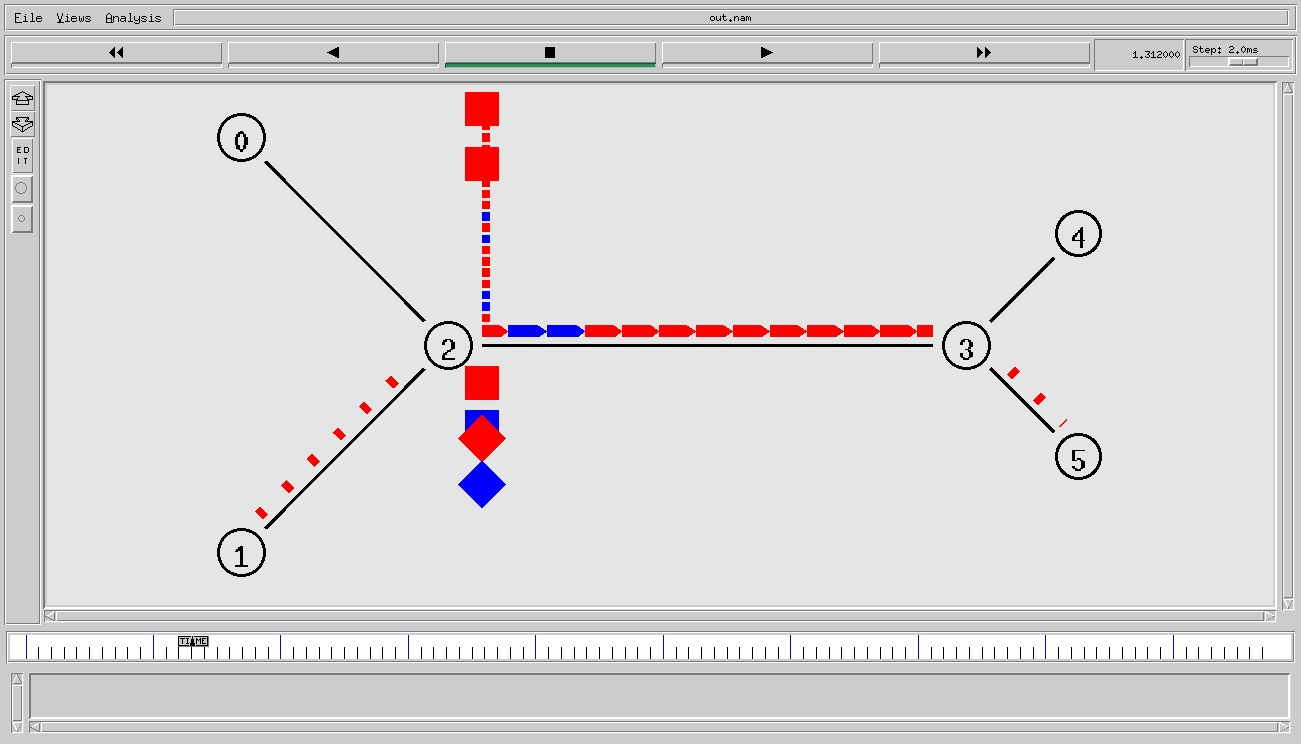
\includegraphics[width=.9\textwidth]{gargalo.jpg}
\caption { Gargalo e perda de pacotes.}
\label{fig:gargalo}
\end{figure}

A figura~\ref{fig:aumentar} mostra um exemplo onde o problema da perda de pacote foi resolvida. O problema foi resolvido através do aumento da banda no enlace n2. Configurada inicialmente com 1 Mb de banda passou a ser de 10 Mb. Com essa nova largura o buffer no nó n2 agora está sendo pouco usado mas a perda de pacote deixou de existir. É importante lembrar que este tipo de solução, aumentando o tamanho do link é cara, o recomendável para um provedor obter melhores lucros com seu link seria a adoção de uma Web cache(ou HTTP cache). Mas para as simulações deste trabalho adotamos como solução para os gargalos aumentar o tamanho do link, até para demostrar o quanto o link teria que ser aumentado caso o provedor prefira investir em uma banda maior em detrimento a uma Web cache.

\begin{figure}[ht]
\centering
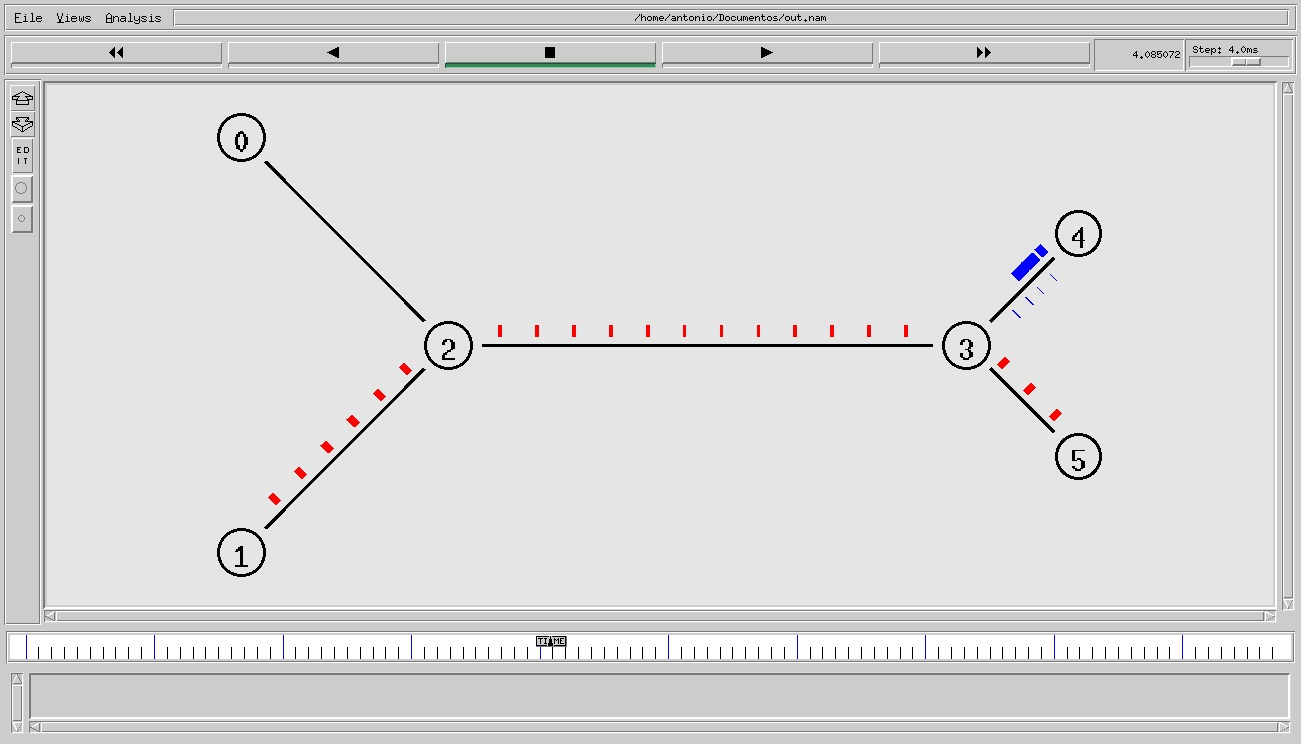
\includegraphics[width=.9\textwidth]{aumentar.jpg}
\caption { Demostração do aumento da banda no enlace n2. Configurada inicialmente com 1 Mb de banda passou a ser de 10 Mb. .}
\label{fig:aumentar}
\end{figure}
\subsection{Anexo do codigo}
 \begin{lstlisting}
set ns [new Simulator]
#Define as cores dos fluxos de dados
$ns color 1 Blue
$ns color 2 Red

#Abre o trace files
set tracefile1 [open out.tr w]
set winfile [open Winfile w]
$ns trace-all $tracefile1
#Faz a analise do arquivo NAM
set nf [open out.nam w]
$ns namtrace-all $nf

#Define o metodo finish, para finalizar o modelo
proc finish {} {
	global ns nf
	$ns flush-trace
	#Close the NAM trace file
	close $nf
	#Execute NAM on the trace file
	exec nam out.nam &
	exit 0
}

#Criando seis nos
set n0 [$ns node]
set n1 [$ns node]
set n2 [$ns node]
set n3 [$ns node]
set n4 [$ns node]
set n5 [$ns node]

#Criando links entre os nos
$ns duplex-link $n0 $n2 5Mb 50ms DropTail
$ns duplex-link $n1 $n2 5Mb 50ms DropTail
$ns simplex-link $n2 $n3 1Mb 100ms DropTail
$ns simplex-link $n3 $n2 1Mb 100ms DropTail
$ns duplex-link $n3 $n4 5Mb 20ms DropTail
$ns duplex-link $n3 $n5 5Mb 20ms DropTail

#Faz a orientacao dos nos (para NAM)
$ns duplex-link-op $n0 $n2 orient right-down
$ns duplex-link-op $n1 $n2 orient right-up
$ns simplex-link-op $n2 $n3 orient right
$ns simplex-link-op $n3 $n2 orient left
$ns duplex-link-op $n3 $n4 orient right-up
$ns duplex-link-op $n3 $n5 orient right-down

#Configura limite de Fila de armazenamento entre link (n2 e n3) para 20
$ns queue-limit $n2 $n3 20
$ns queue-limit $n3 $n4 20

#Monitorar a fila para link (n2-n3), (n3-n4) e (n3-n5). (para NAM)
$ns duplex-link-op $n2 $n3 queuePos 0.5
$ns duplex-link-op $n3 $n4 queuePos 0.5

#Configurar a conexao TCP
set tcp [new Agent/TCP]
$tcp set class_ 2
$ns attach-agent $n0 $tcp
set sink [new Agent/TCPSink]
$ns attach-agent $n4 $sink
$ns connect $tcp $sink
$tcp set fid_ 1
$tcp set packetSize_ 1024

#Configurar um FTP sobre conexao TCP
set ftp [new Application/FTP]
$ftp attach-agent $tcp
$ftp set type_ FTP

#Configurar a conexao UDP
set udp [new Agent/UDP]
$ns attach-agent $n1 $udp
set null [new Agent/Null]
$ns attach-agent $n5 $null
$ns connect $udp $null
$udp set fid_ 2

#Configurar um CBR sobre conexao UDP
set cbr [new Application/Traffic/CBR]
$cbr attach-agent $udp
$cbr set type_ CBR
$cbr set packet_size_ 1024
$cbr set rate_ 1Mb
$cbr set random_ false

#Delimitacao do eventos para agentes CBR e FTP
$ns at 0.1 "$ftp start"
$ns at 0.4 "$cbr start"
$ns at 4.0 "$cbr stop"
$ns at 4.5 "$ftp stop"

proc plotWindow {tcpSource file} {
	global ns
	set time 0.1
	set now [$ns now]
	set cwnd [$tcpSource set cwnd_]
	puts $file "$now $cwnd"
	$ns at [expr $now+$time] "plotWindow $tcpSource $file"
}

$ns at 0.1 "plotWindow $tcp $winfile"

#Chamar o metodo finish apos 5 segundos de tempo de simulacao
$ns at 5.0 "finish"

#Apresente o tamanho do pacote e intervalo CBR
puts "CBR packet size = [$cbr set packet_size_]"
puts "CBR interval = [$cbr set interval_]"

#Executar a simulacao
$ns run


\end{lstlisting}

\section{Graphical Network Simulator}


É um emulador de Software que permite a combinação de dispotitivos reais e virtuais, usado para simular redes complexas. O GNS3(Graphical Network Simulator-3) permite o mesmo tipo de
emulação usando os sistemas operacionais Cisco Internetwork. Permite que você possa executar um Cisco IOS(Internetwork Operating System) em um ambiente virtual em seu computador. GNS3 é uma frente gráfica para um produto chamado Dynagen. Dynamips é o
programa principal que permite a emulação IOS. O GNS3 dá um passo adiante ao fornecer um ambiente gráfico.

O GNS3 permite a emulação de IOS da Cisco no Windows ou no Linux. A emulação é possível para uma longa lista de plataformas de roteador e PIX
firewalls. Usando um cartão EtherSwitch em um roteador, as plataformas de comutação também podem ser emuladas ao grau do cartão da funcionalidade suportada. Isso significa que GNS3 é uma ferramenta inestimável para
preparação de  certificações da Cisco, como CCNA e CCNP. 

Com GNS3 você estará executando um Cisco IOS real, então você verá exatamente o que o IOS produz e terá acesso a qualquer comando ou parâmetro suportado pelo IOS. Além disso, o GNS3 é um programa aberto e gratuito para você usar. 
\subsection{Instalação}
A instalação do simulador GNS3 foi feita por linha de comando no sistema operacional linux (Ubuntu 16.04). Além deste pacote, foi instalada os pacotes de roteadores necessários para a correta manipulação do simulador.

Após a instalação a configuração foi feita de acordo os parâmetros requeridos. feitos os testes, a instalaçãoo foi concluída sem erros.
\subsection{Problemática} 
Suponha que uma escola de ensino fundamental necessite colocar os computadores do seu novo Laboratório Escolar de Informática – LEI em rede, além dos computadores da diretoria e secretaria. Para fazer isso precisa comprar uma serie de equipamentos. Sabemos que órgãos públicos precisam fazer licitações para adquirir qualquer bem. Então como saber qual a lista de equipamentos que precisam ser comprados sem correr o risco de sobrar equipamento causando prejuízos ao erário público ou faltar equipamentos e não conseguir montar a rede? 

Diante disto surge o GNS3 capaz de simular toda estrutura da rede, possibilita a realização de testes, ilustrar cada periférico da rede, entre outras funcionalidades. Com todos estes recursos pode se testar varias estruturas de rede para escola, até encontrar a ideal  e simplesmente adquirir todos os equipamentos que foram utilizado na versão ideal da estrutura da rede. 
\subsection{Simulação}
A simulação que fizemos trata-se de uma rede de computadores de uma escola. Criado o ponto de acesso, um roteador foi colocado para distribuir a conexao entre o ponto de acesso e a diretoria, secretaria e o laboratório.
\begin{figure}[ht]
\centering
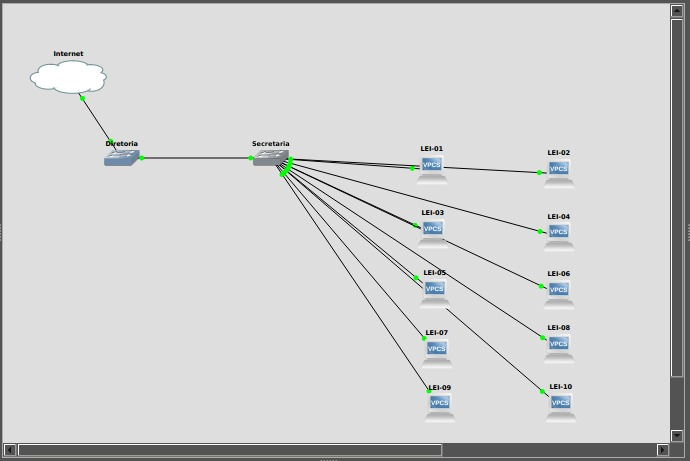
\includegraphics[width=.9\textwidth]{internet.jpeg}
\caption { Demonstração da rede da escola simulada no GNS3.}
\label{fig:gargalo}
\end{figure}
O roteador da diretoria envia o sinal para o roteador da secretaria, que distribui para o laboratório.

A simulação dessa rede é visualizada no próximo tópico
\subsection{Resultados}
Conseguimos ilustrar a rede da escola,e concluimos que os unicos equipamentos necessários foram dois swichts. Bom sabemos que algo tão simples não necessitava de um simulador para desenvolver a estrutura desta rede, mas o intuito era mostra a funcionalidade da ferramenta. Sabendo que em uma estrutura de rede grande ela seria indispensavél.   
\begin{figure}[ht]
\centering
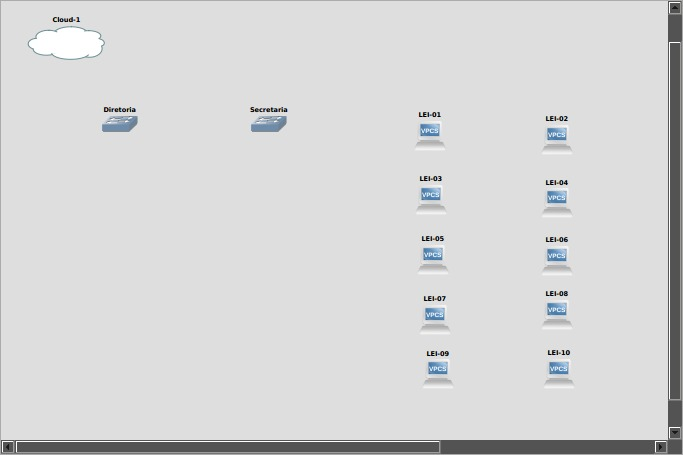
\includegraphics[width=.9\textwidth]{estrutura.jpeg}
\caption { Demonstração da rede da escola simulada no GNS3.}
\label{fig:gargalo}
\end{figure}

\section{Considerações Finais}\label{sec:figs}
 Os simuladores são alternativas ótimas para projetos com uma estrutura orçamentário bem limitada para a representação física de uma rede de computadores. Eles acabam por propiciar uma forma eficiente de testes, e levantamento de custo, reduzindo o máximo possível de desperdício.
 
Um dos simuladores que abordamos foi o NS2 que atualmente é manuseado por vários grupos de pesquisa, por alunos que desejam mais conhecimento em redes, em corporações de redes sem fio, celulares, satélite, simulação de ataques de Negação de Serviço (Denial of Service - DoS) para testes de segurança.

Como nosso exemplo na simulação mostrou, para quem entende o básico do funcionamento de uma conexão de redes de computadores, pudemos, após analisar os dados dos enlaces, resolver um problema que é corriqueiro no nosso meio.

O simulador NS2 é praticamente uma ferramenta indispensável para os profissionais da área, pois oferece tipos variados de simulações, minimizando os problemas que uma rede de computador está sujeita.
\bibliographystyle{sbc}
\bibliography{sbc-template}

\end{document}
